
%%%%%%%%%%%%%%%%%%%%%%%%%%%%%%%%%%%%
\chapter{Methodology}
\label{chap:Methodology}

To our knowledge, the deep learning networks and architectures adaptations review in \ref{chap:Literature_Review} only include traditional hand-crafted approaches and adaptions of various vanilla backbone architectures. Almost all approaches formulate problems as binary classifications and reproduce overall accuracy. There are two approaches to this: thresh-holded MOS prediction(regression) models output, and training pre-thresholded classes by GT MOS, both with a test train split applied by \cite{Talebi2018,Murray2012}. 

Here, we adopt the latter as a more challenging problem with a clear relationship to real world applications of IAQA and less room for ambiguity within the accuracy metrics (which the authors observe in some of the IAQA literature). 

Some approaches appear to present the accuracy of a ten class (model) MOS, which will give higher accuracy on test data as the trained network will not have to tolerate fully the significant number of images with MOS very close to the high-low class threshold. Further, with a 2 node output vs 10 node there are quite simply 5 times less gradients to vanish. 

Here, we train a various transformer models - both vision transformer ViTs and convolutional vision transformer CvTs. The reasons for this are: \begin{enumerate}
    \item Transformers have not yet been applied to IAQA and a side-by-side comparison generates new insights;
    \item Many deep learning models have relied on hand-crafted attention mechanisms, a process which is a learned intrinsic feature of Vision Transformer(ViT);
    \item Many more recent models have combined deep features with attention layers to obtain the best of both worlds;
    \item There exist a number of pre-trained models on imagined allowing efficient transfer learning to and IAQA Domain.
\end{enumerate}

\subsection{Side By Side Comparisons}
\label{side by side}
Vision transformers require huge datasets and special treatment via custom training schedulers, which have warm-up and cool-down data phases. 

Comparing ViTs, CvTs and CNNs side-by-side on as close as possible training conditions enables an evaluation of whether the introduction of convolution is a means to soften the hard requirements of ViTs during training, providing inductive bias inherent in CNNs. 

We reproduce an example to illustrate how CNNs convolve and maintain spatial proximity. Red shows the kernel and green bounding box shows the image area covered; here, kernel size and stride are parameters that effect feature maps learned. 

\begin{figure}
    \centering
    \begin{subfigure}[b]{0.2\textwidth}
        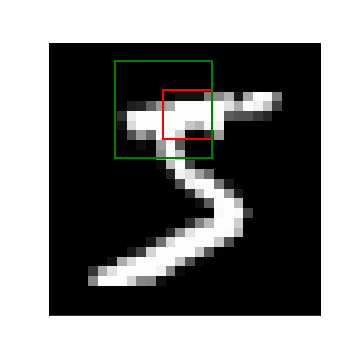
\includegraphics[width=\textwidth]{figures/research_methadology/mnist_five.png}
        \caption{5 from MNIST Handwriting Dataset \cite{LeCun1998}}
        \label{fig:MNIST 5}
    \end{subfigure}
    \hspace{10mm}
    \begin{subfigure}[b]{0.2\textwidth}
        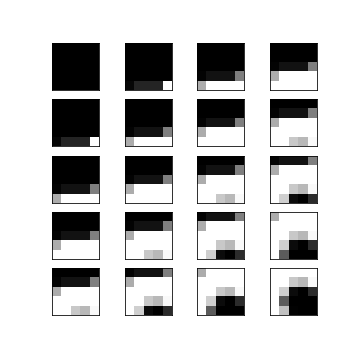
\includegraphics[height=\textwidth]{figures/research_methadology/mnist_five_convolved.png}
        \caption{\textbf{Convolutions} Filter Kernel of Size (5,5) Stride of (5,1)}
    \end{subfigure}
    \hspace{10mm}
    \begin{subfigure}[b]{0.2\textwidth}
        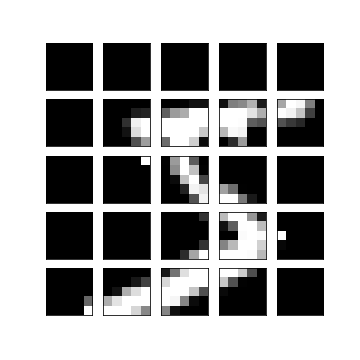
\includegraphics[height=\textwidth]{figures/research_methadology/mnist_five_patched.png}
        \caption{\textbf{Patches} Filter Kernel of Size (5,5) Stride (5,5)}
    \end{subfigure}
    \caption{Illustration of Spatial Inductive Bias}
    \label{fig:Inductive Bias EG}
\end{figure}

Contrast this with figure \ref{fig:CvT}: patches are exclusive and then attention is learned between \textit{tokenized} discrete patches- clearly a very different paradigm.

We employ domain adaption as an overall approach, where target domain is IAQA binary classification and source domain is multi-class classification convolution architectures of both convolution and ViT models. This brings with it the further strength of being able to use pre-trained models, which do not require compute intensive training from scratch. Transformers require large datasets\cite{Zhang2021,Kolesnikov2020,DAscoli2021,Khan2021,xiao2021early,Wu2021} with then hundreds of millions of labelled data entries\cite{Zhang2021} to converge and produce state of the art metrics, which is much larger than required for CNNs. This is at least in part because CNNs encode prior knowledge (adapting stride and kernal size) of image domain such as \textit{translation equivariance} \cite{Khan2021} across feature maps (figure \ref{fig:Inductive Bias EG} illustrates one example of this), CvTs do not have this as a possible prior embedding; these must be fully learned across discrete patches. Various approaches have been used to improve performance, such as introduction of gated position self-attention (GPSA)\cite{Touvron2021a,Touvron2020a,DAscoli2021}. We will use domain, adaptation, and transfer learning as well as improvements to data requirements that have been introduced. This section will cover our approach on the following areas: \begin{enumerate}
    \item Transformer Architecture
    \item Pipeline and Pre-Procession
    \item{Data Augmentation}
    \item Training Methodology
    \item Testing Methodology
\end{enumerate}



\section{Transformers}
\label{Transformeres} 
Transformers have come to dominate over the recent years in many domains, have outperformed Convolutional Neural Networks (CNN), Recurrent Neural Networks (RNN) such as Long and Short Term Memory (LSTM) architecture\cite{Vaswani2017a} and have become a hot topic. 

Many of these were designed to address challenges such as vanishing gradients, and in many areas, this began with applications such as machine translation within natural language processing (NLP)\cite{Wolf2020a}. These were also areas where attention mechanisms have become an integral part\cite{Vaswani2017a}. 

The transformer consists of blocks (head) in which each learner in sequence learns alignment in K, a value query system where input $Q$is passed to an embedding layer One-Hot tokenization. Input is a tensor of shape $\mathbb{R}^B \times \mathbb{R}^N \times \mathbb{R}^D$ where B is batch size, N is sequence length, and D is dimensional embedding.\cite{Tay2020}. Each attention model architecture can be seen in figure \ref{fig:Vaswani2017a_trans_arch}
\begin{figure}
    \centering
    \begin{subfigure}[b]{0.3\textwidth}
        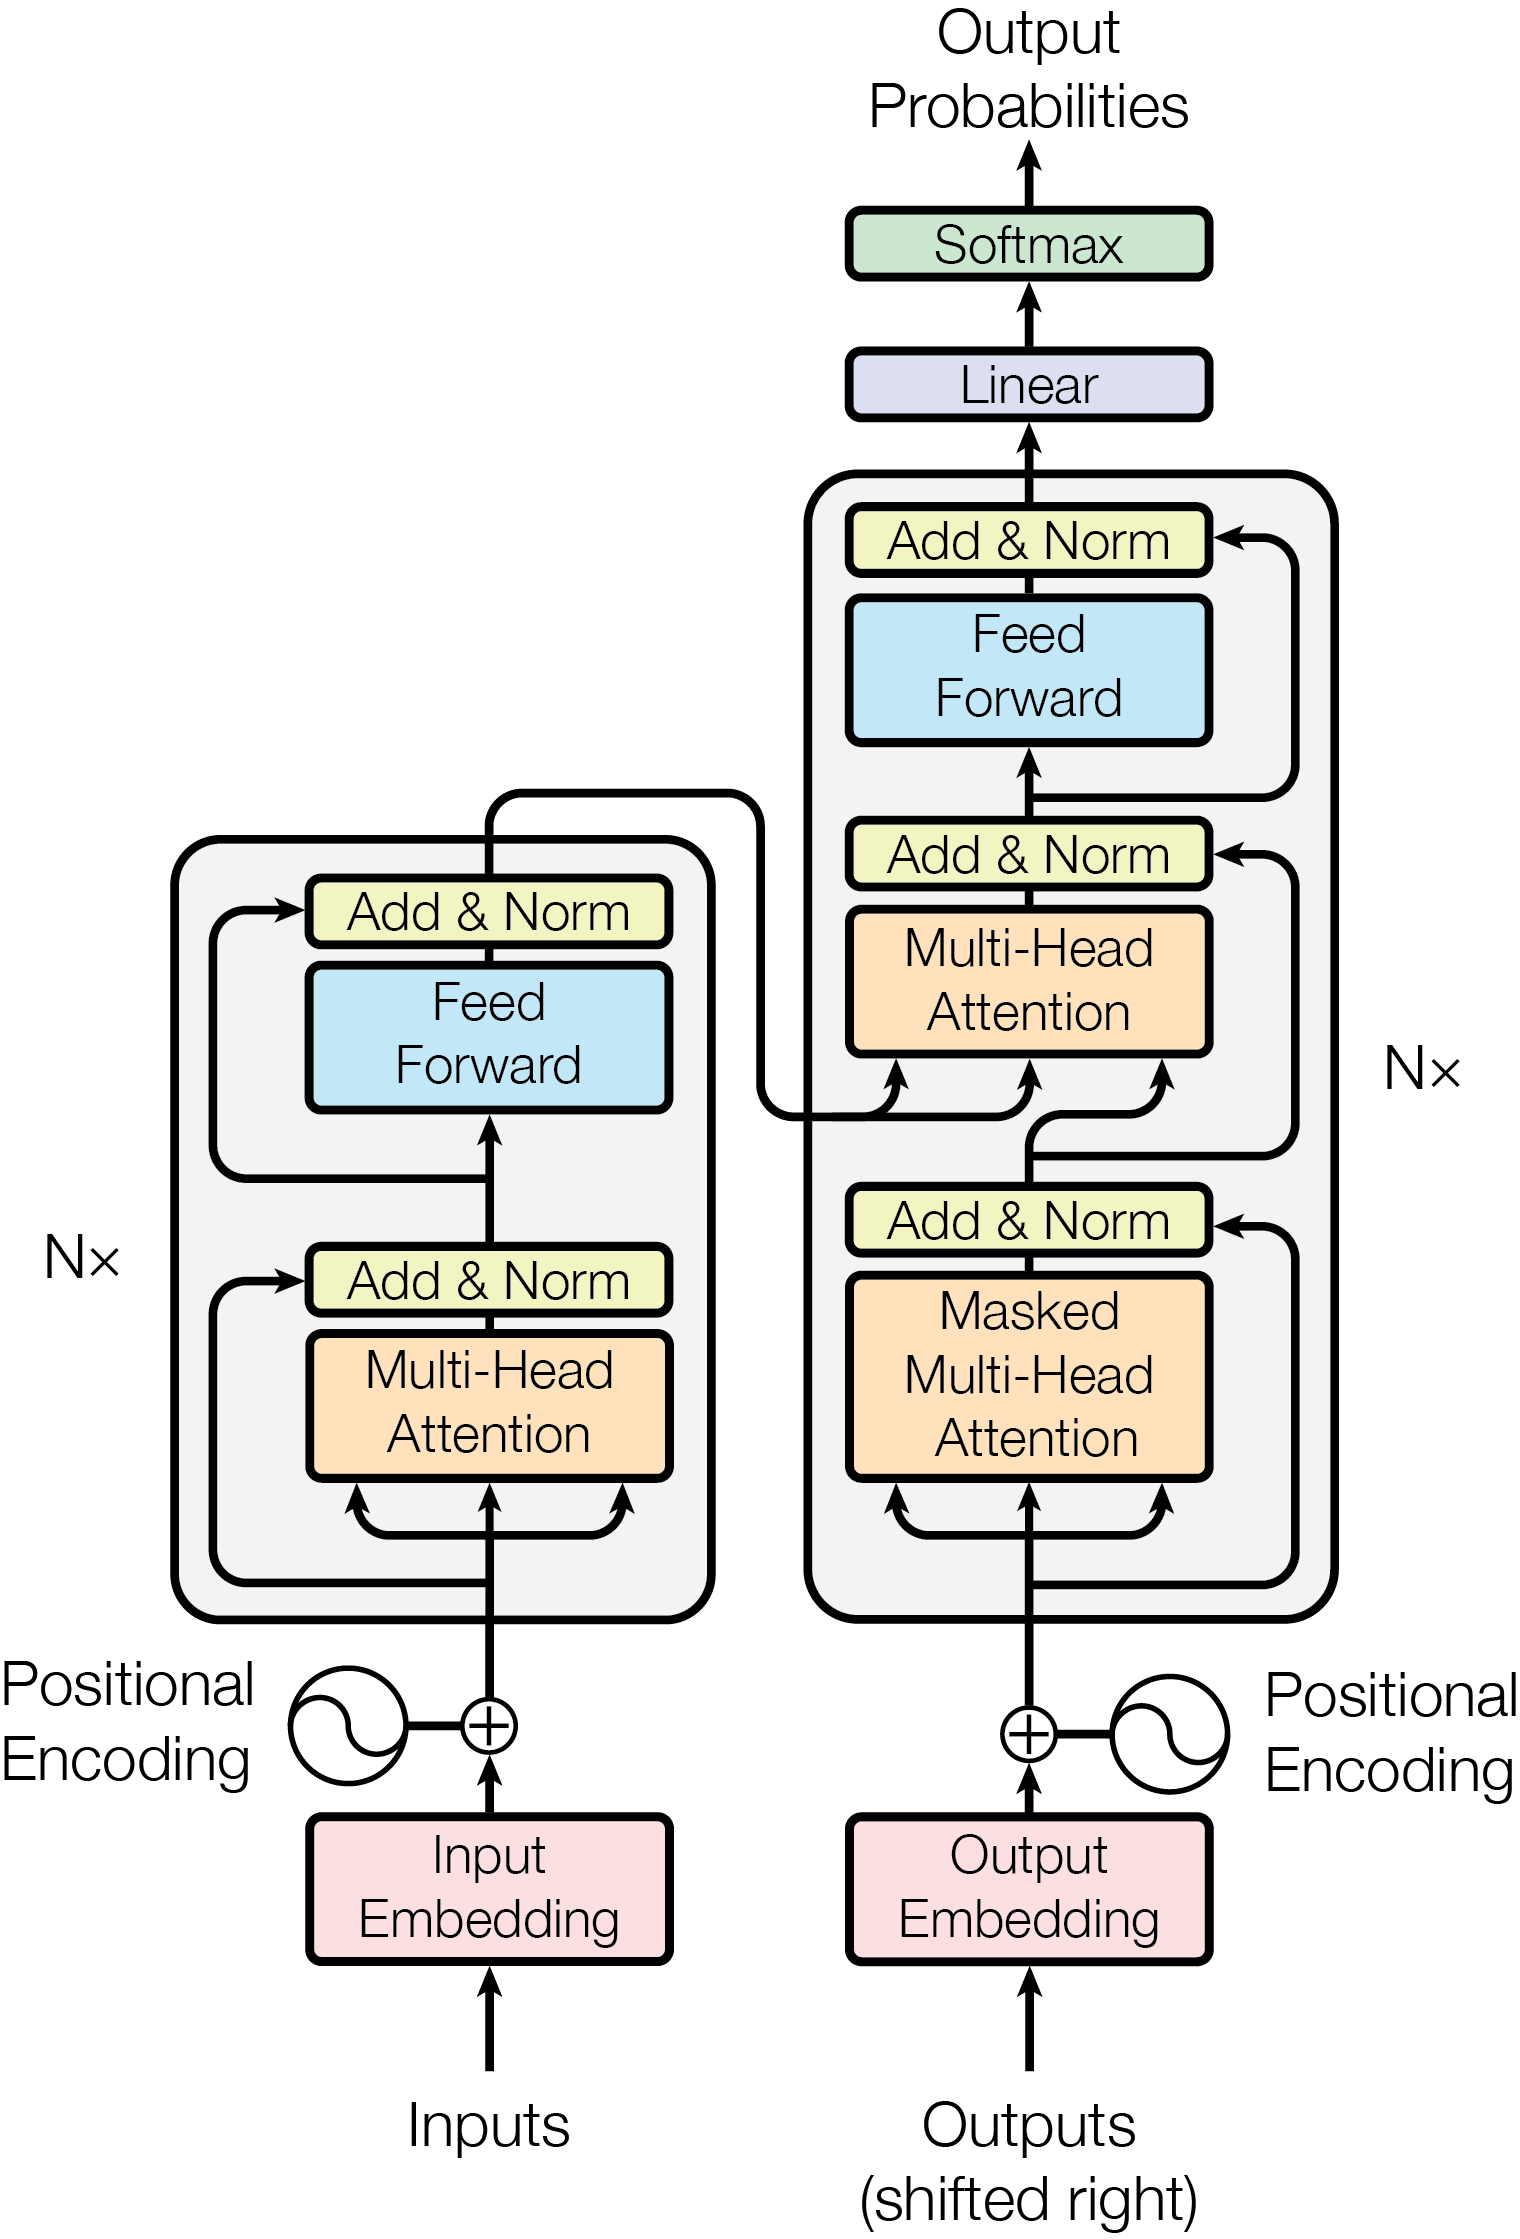
\includegraphics[width=\textwidth]{figures/research_methadology/tranformer_architecture.png}
        \caption{Attention Model Architecture \cite{Vaswani2017a}}
        \label{fig:Vaswani2017a_trans_arch}
    \end{subfigure}
     \hspace{10mm}
    \begin{subfigure}[b]{0.3\textwidth}
        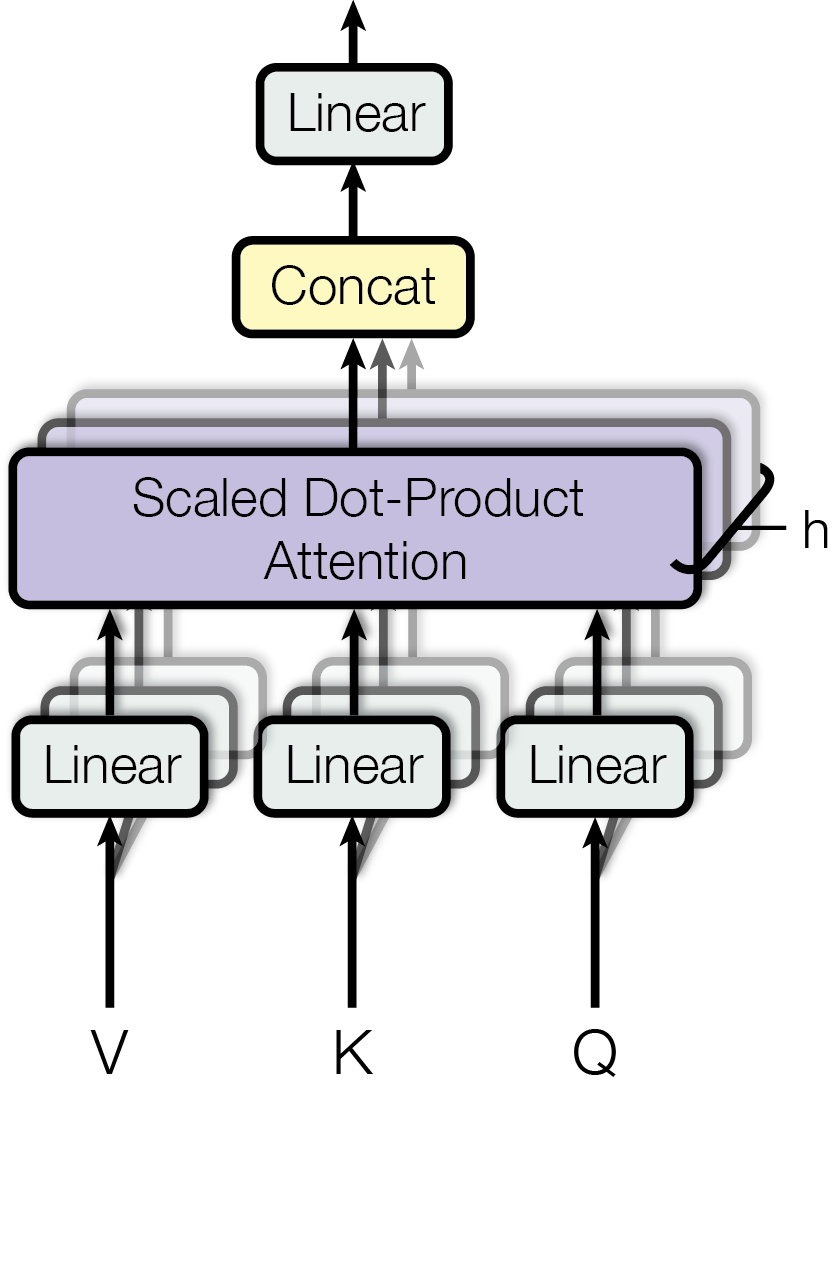
\includegraphics[height=\textwidth]{figures/research_methadology/multi-head attention.png}
        \caption{Multi Head Attention  \cite{Vaswani2017a}}
        \label{fig:Vaswani2017a_attention}
    \end{subfigure}
    \caption{Initial Attention Model Diagram}
    \label{fig:transformers}
\end{figure}

\subsubsection{Self Attention\label{Attenion_s}}
Attention is is a mapping of query ($Q$), key ($K$), value ($V$) pairing - this is not unlike the python dictionary with a key store. V, K, Q are $MxN$ square matrices. The matrix Q is the product of the computation of a set of queries with all keys\cite{Vaswani2017a} $d_k$ and values $d_v$.  Attention output is given by:

\begin{equation}
    Attention(Q,K,V) = Sotftmax(\dfrac{QK^T}{\sqrt{d_k}})V
\end{equation}

Where $D_k$ is the radical(square root) of the number of patches, a process which avoids vanishing gradients. This attention function is performed in parallel for each head, and these are concatenated back and re-projected. Figure\ref{fig:Vaswani2017a_attention}, the resulting linear output depicted in figure \ref{fig:Vaswani2017a_trans_arch} immediately before softmax layer, which produces class probability. What is learning in this process are linear projections, first local in parallel (each attention head) and then through global projection, produce final values given by:
\begin{equation}
    MultiHead(Q,K,V) = Concat(h_1,...,h_n)W^O
\end{equation}
Where $h_i = QW^Q_i,KW^K_i,VW^V_i$ or the application of attention function to the $i_{th}$ where parameters of multi-head function  are $W_i^Q\in \mathbb{R}^{d_{mdl.}\times d_k},W_i^K \in \mathbb{R}^{d_{mdl.}\times d_k},W_i^V \in \mathbb{R}^{d_{mdl.} \times d_v}, W^O \in \mathbb{R}^{d_{mdl.} \times hd_v}$. Note the last parameter passed is effectively a $O_th$ where $h$ is the number of attention layers\cite{Vaswani2017a}, which is, in effect, a high-level recursive application where power law applies to recursion depth. 

\section{Vision and Convolution Transformers\label{transformer_method}}
\label{ConViTs} 

Here, we initially train Vision Transformers (ViT) - which were adapted as closely as possible from \cite{Vaswani2017a}'s application within NLP by \cite{Dosovitskiy2020} for image classification, a high-level overview can be seen in figure\ref{fig:ViT}. Changes are additional for the final MLP. \cite{Dosovitskiy2020} also shows that attention head can be mapped onto convolutional feature maps. 

Both require flattening of images into 2D exclusive patches $x\in{\mathbb{R}^{H\times W \times C}}$ where $C$ is the number of channels; $H,W$ are the input image height and width; $N$ is patches of image resolution; ($H\times W$) is the resolution dimension of $P^2$ where $W=H$. This is simply $N = \dfrac{W^2}{P^2}$. 

The embedding process that \cite{Dosovitskiy2020} introduces is token embedding $\textbf{E}$  where $\textbf{E}\in\mathbb{R}^{(P^2C)\times D}$  (where $D$ is vector size) and positional embedding $\textbf{E}_{pos}\in\mathbb{R}^{(N+1)}$, which is added to patch embedding to retain position information given by:

\begin{equation}
    Z_O = \begin{bmatrix}
    \textbf{x}_{class};& \textbf{x}^1_p\textbf{E};& \dotsm \ ; & \textbf{x}_p^N\textbf{E} 
    \end{bmatrix} + \textbf{E}_{pos}
\end{equation}

Where $\textbv{E}_{pos}$ is learnable positional embedding shown in dark pink in figure \ref{fig:ViT}, and is added to the concatenated patch embedding(s) back to a final $1\times n$D Vector, hence both global and local self attention can be learned. 

\begin{figure}[h!]
    \centering
    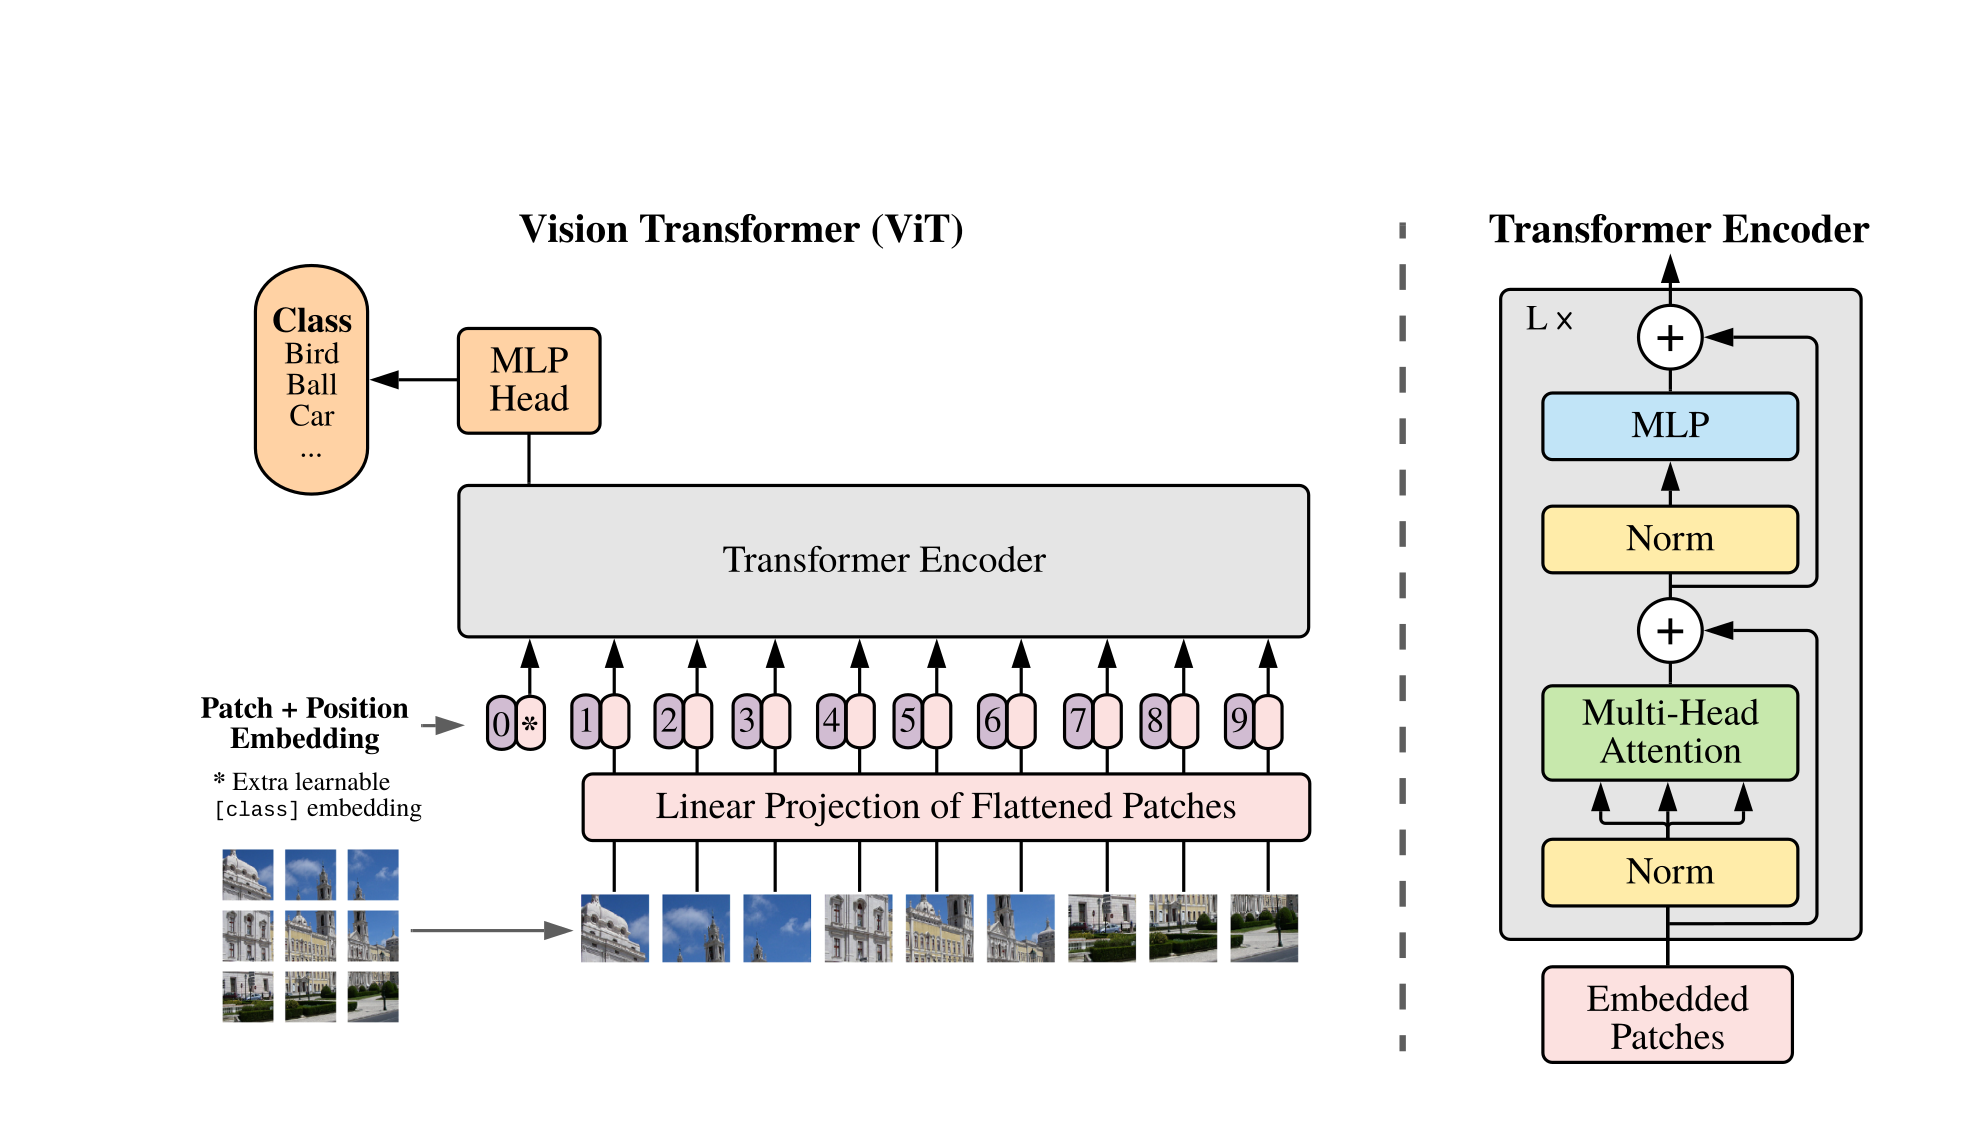
\includegraphics[width=0.8\textwidth]{figures/research_methadology/Dosovitskiy2020_VIT.png}
    \caption{High level overview of Initial Implementation of ViT  \cite{Dosovitskiy2020}}
    \label{fig:ViT}
\end{figure}

\newpage

\subsection{Training Approach}
Transformers require extremely large amounts of data to train, $10 \times$ typically larger than any available IAQA dataset. We combat this in three ways:
\begin{description}
    \item[Transfer Learning] leveraging transformers have been trained on ImageNet1k\cite{Ridnik2021};
    \item[Data-efficiency] using state of the art(SOtA) data efficient transformers\cite{DAscoli2021,Touvron2021a} that are able to train on smaller datasets that have been able to train on subsets of ImageNet1K; 
    \item[Augmentation] using SOtA\cite{Buslaev2020a,Riba2020} approaches such as reflection padding; 
\end{description}
We use pre-trained data efficient transformers developed by \cite{Touvron2020a} models on image net, which introduces soft inductive biases (initialization patches through convolution) developed by \cite{DAscoli2021} and keeping input dimension unchanged at $3 \times 224 \times 224$. Images are resized from the original to the longest edge. In order to preserve computational information, we train on both zero-padded and reflection padded images, where images are grey-scale $224 \times 224$ these are stacked to three equal channels as a simple means to ensure bias is not introduced to the model. We train models of three sizes, of modified data efficient transformer ConViT $\in \{Ti,S,B\}$, which are\cite{DAscoli2021}'s adaptions of DeiT-Ti,DeiT-S,DeiT-B\cite{Touvron2020a}.

\begin{table}[]
    \centering
    
    \begin{tabular}{p{2cm}<{\centering}|p{2cm}<{\centering}c{1.5cm}c{2cm}c{2cm}c{2cm}}
    \specialrule{.1em}{.05em}{.05em} 
         Model & Embedding Dimension & Heads & Layers& Params & Image Resolution   \\
    \specialrule{.1em}{.05em}{.05em} 
    ConViT-Ti & 192 & 3 & 12 & 5M & $224 \times 224$\\
    ConViT-S & 238 & 6 & 12 & 22M & $224 \times 224$\\
    ConViT-B & 768 & 12 & 12 & 86M & $224 \times 224$
    \end{tabular}
    \caption{Efficient ConVits trained adapted from \cite{Touvron2020a,} }
    \label{tab:ConViTs}
\end{table}

The models have a final, fully connected layer of $[1 \times 1000]$ classes, and therefore we add a fully connected layer of $[1 \times 2]$ using PyTorch \lstinline[columns=fixed, language=Python]{nn.Layer(1000,2)} to add a finally fully connected layer to the ConViTs model. We trained ConViT-Ti using a formative grid search, as a new hyper parameter is introduced as a modified Deit-Ti model. This requires significant search, and therefor we only perform a grid search on ConViT-Ti. Trained adjusting hyper parameters incrementally within grid searches for 10 approaches. We also train ConViTs $\in \{Ti,S,B\}$ shown inn Table \ref{tab:ConViTs} with no changes to hyper parameters to provide insights into how including embedded dimension, number of attention heads effects performance on test set. Finally, we train the best model on the best performing hyper parameters. 

\pagebreak  

\subsection{Augmentation} 

%%% transform = transforms_imagenet_train(hflip=hflip,
%                vflip=vflip,
%               color_jitter=color_jitter,
%    
%                std=std,
%                re_prob=re_prob,
%                re_mode=re_mode,
%                re_count=re_count,
%                re_num_splits=re_num_splits,
%                separate=separate)

Data Augmentation is an important part of regularisation in deep learning \cite{Kukacka2017}; it is a powerful way to mitigate against over-fitting during training and supports better generalization\cite{Shorten2019} - ensuring that validation error decreases with training error, we implement conventional methods\cite{Mikolajczyk2018} alongside state of the art methods proposed by\cite{Riba2020,Buslaev2020a}. 

\par

Here, augmentation of images is in two stages: first, all images are square padded to zero to preserve com positional information, or reflection padded\cite{Buslaev2020a} and resized to $3 \times 224 \times 224$. Larger image configurations are possible, however for consistency in baseline comparisons and IAQA approaches we maintain this a base dimension.  During training, we augment applying random occlusion/erasure of images to remove a random patch of image for $16\times16$ pixels, random rotation, spatial transforms such as shear and colour-gitter, gaussian noise (5,5) filter and gaussian blur (5,5) filter in addition to square distortions. 

We also use occlusion patches randomly applied to images of the same dimension of image patches, this is to strategically remove patch sized areas of the image while allowing the model to train attention on other areas of the image. 


\begin{figure}[ht!]
    \centering
    \specialrule{0.01em}{1em}{1em}
\begin{subfigure}[b]{0.2\textwidth}
    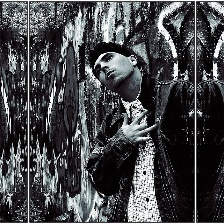
\includegraphics[height=\textwidth]{figures/research_methadology/augmentation/112197.jpg}
    \label{reflection_pad}
    \caption{Reflection Padding to $224 \times 224$  with Albumentations}
\end{subfigure}
\hspace{10mm}
\begin{subfigure}[b]{0.2\textwidth}
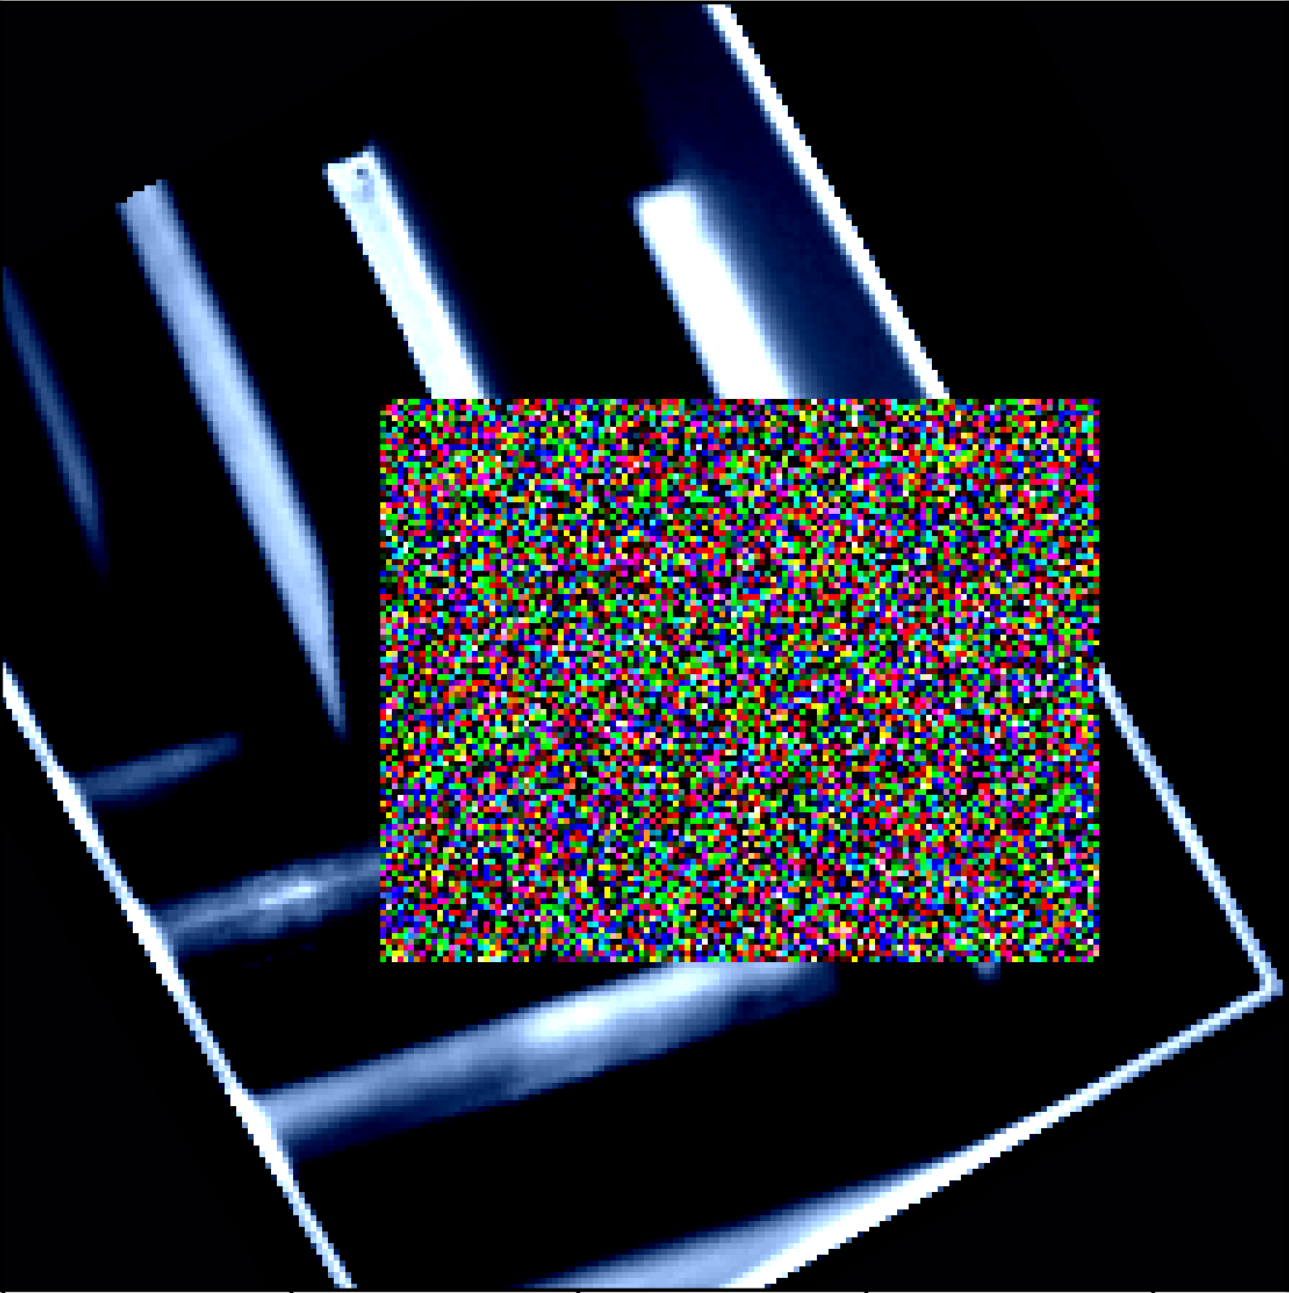
\includegraphics[width=\textwidth]{figures/research_methadology/augmentation/train_augment.png}
\label{Train_augment}
\caption{Training Augmentation Rotates and Random Erasure/Occlusion}
\end{subfigure}
\hspace{10mm}
\begin{subfigure}[b]{0.2\textwidth}
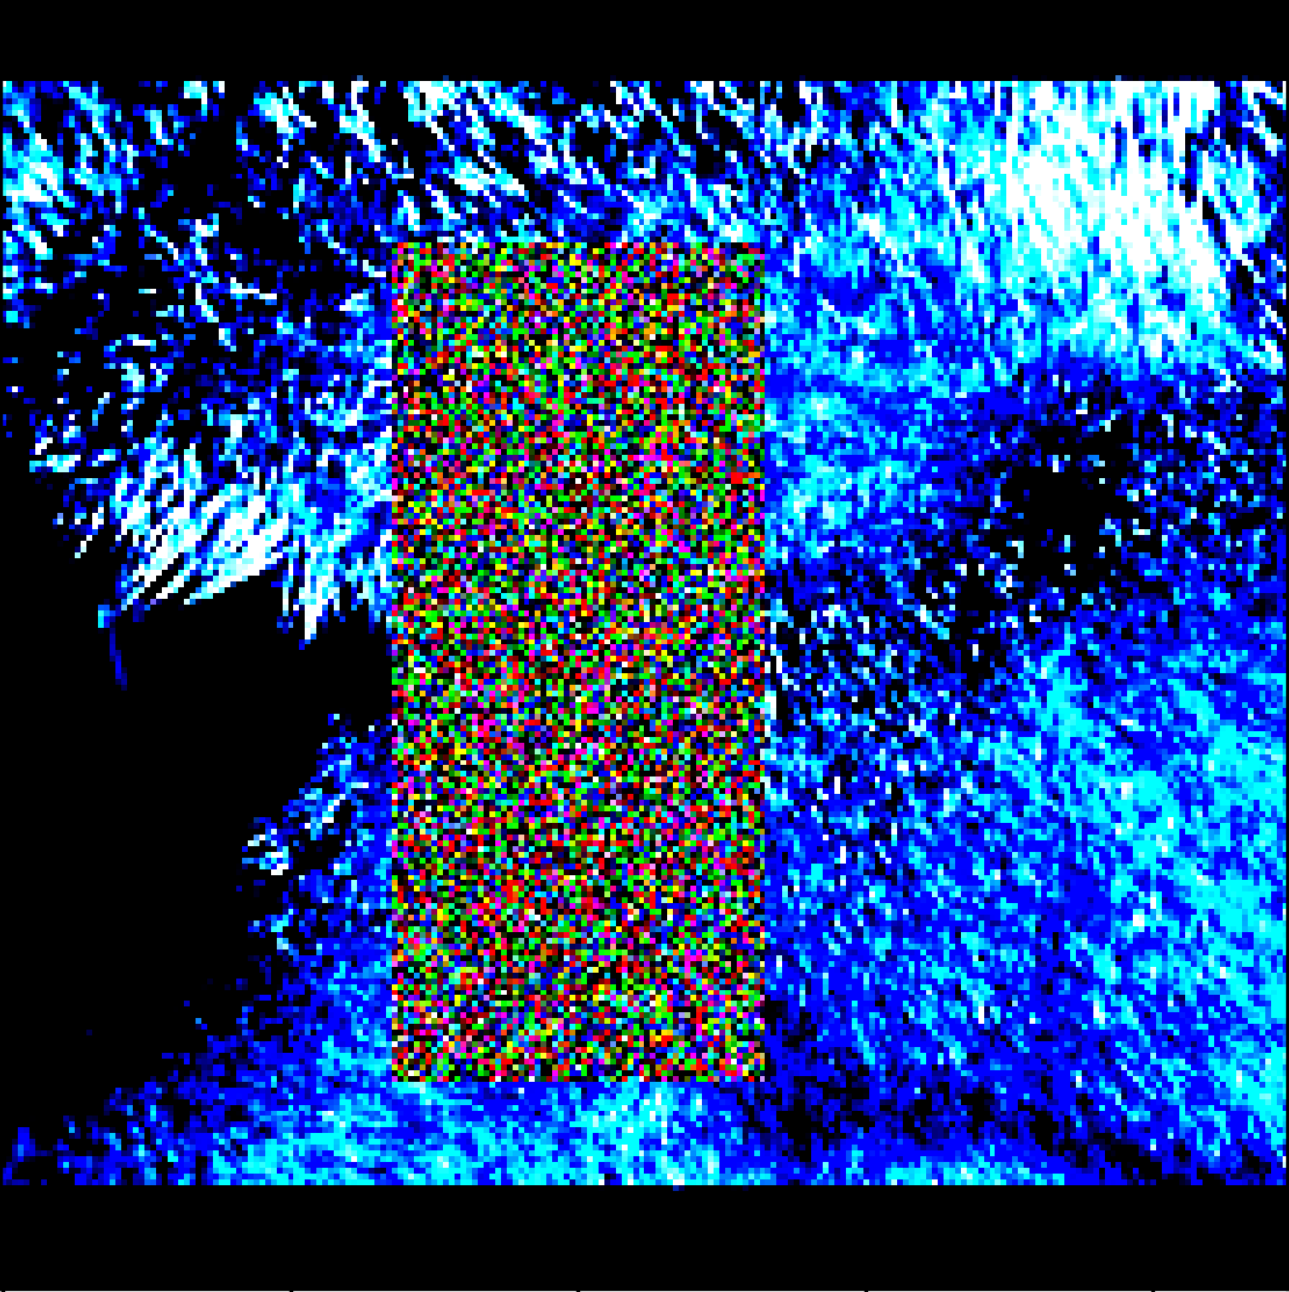
\includegraphics[width=\textwidth]{figures/research_methadology/augmentation/train_augment_2.png}
\label{Train_augment_2}
\caption{Training Augmentation Zero Padding, Random Erasures}
\end{subfigure}
    \caption{Augmentation Examples}
    \label{fig:aumentation}
\specialrule{0.01em}{1em}{1em}
\end{figure}


\subsection{Data Preprocessing and Normalization}
An essential part of optimising learning, both to improve training results and ensure consistency of method elsewhere.  All image  normalising using image change $\in\{R,G,B\}$ mean given by:

\begin{equation}
    \mu = \dfrac{1}{n}\sum^n_1x_i
\end{equation}

And standard deviation given by:

\begin{equation}
    \sigma^2 = \dfrac{1}{n}\sum^n_i^2-\mu^2
\end{equation}
 
Where n is number of pixels and $x_i$ is $i_{th}$ a pixel value of 0-255. 

Resulting tensors are 32-bit floating points (FP) between 0-1, mean and standard deviation  RGB values $\mu = 0.485, 0.456, 0.406$, $ \sigma = 0.229, 0.224, 0.225$.

\subsubsection{Ground Truth Discretization}

AVA ground truth is derived by two processes. MOS scores are in categories $1-10$ the MOS  can be computed neatly by: 
\begin{equation}
    \mu = \sum_{i=1}^n a_i\cdot b_i^T
    \label{mos}
\end{equation}
Where $a$ is a normalised vector of scores and $b$ is a sequence vector $1-n$ \footnote{Presented in this way for conceptual clarity and to resemble as closely as possible Python's numpy operations}. Mean scores are then thresholded by: 
\begin{equation}
  {s} =
    \begin{cases}
      1 & \geq \mu \geq 5 \leq 4\sigma\\
      0 & \leq \mu \leq 5 \leq 4\sigma\\
    \end{cases}
    \label{eq:threshold} 
\end{equation}

Where $\mu$ is given by eq. \ref{mos} and $\sigma$ is standard deviation of overall MOS scores. This results in a small number of outliers (just 97 images out of 255508) excluded from training, test and validation sets; for many within the literature the convention is exclusion of MOS $\pm 4\sigma$. 

\subsection{Hyper Parameter Search}

We perform several grid searches of hyper parameters by defining a function called within a training class that initialises existing code using Python's inbuilt sub process module, which augments rather than rebuilds the model.

The purpose of a conduction grid search is not to comprehensively tune the base model, but to assess how newly introduced hyper parameters (`locality strength' and `locality up to layer') which incorporate convolutional inductive bias effectively adapt the model to the target domain.

This is for methodological consistency, and to enable tuning of newly introduced softer inductive bias GPSA\cite{DAscoli2021}. The assumption made is that a degree of due consideration is made by \cite{DAscoli2021,Touvron2021a}.

Training time for 10 epochs is 25 minutes; where unique parameter combinations are used, this was a total 3 days per grid search and also involved ensuring that the model can be reinitialised. Weights were saved for every epoch of each model in the grid search. 

\begin{table}[ht!]
\small 
    \centering
    \begin{tabular}{c?cc}
    \toprule
         parameters & Constraints & Intervals \\
         \midrule 
         locality strength & 0.5-1.5
         & 10\\
         learning rate & 0.001-3&3\\
         \bottomrule
    \end{tabular}
    \caption{Formative Grid Search Parameters}
    \label{tab:hyper_params}
\end{table}
\subsection{Test Train Validation}

We employ a test train split defined within the literature\cite{Murray2012}. For convenience, \cite{Talebi2018} have made available a .csv file which has image references alongside test, training and validation images. For the reproduction of results and methodological clarity, we have also made available .json files of test image IDs. $\in\{test,train,validation\}$ image numbers are \textbf{19928, 223795, 11779}. Figure \ref{fig:test train} shows a bar plot of $\in\{test,train,validation\}$ sets.





%\subsection{Domain Adaptation}

\subsection{Models}
We train from/create several transformer models built on \cite{Touvron2020a}'s DeiT, with added GPSA\cite{DAscoli2021} and \cite{Wu2021}, figure \ref{fig:ConViT model} show addition of GPSA at local level. 

\begin{figure}[ht!]
    \centering
    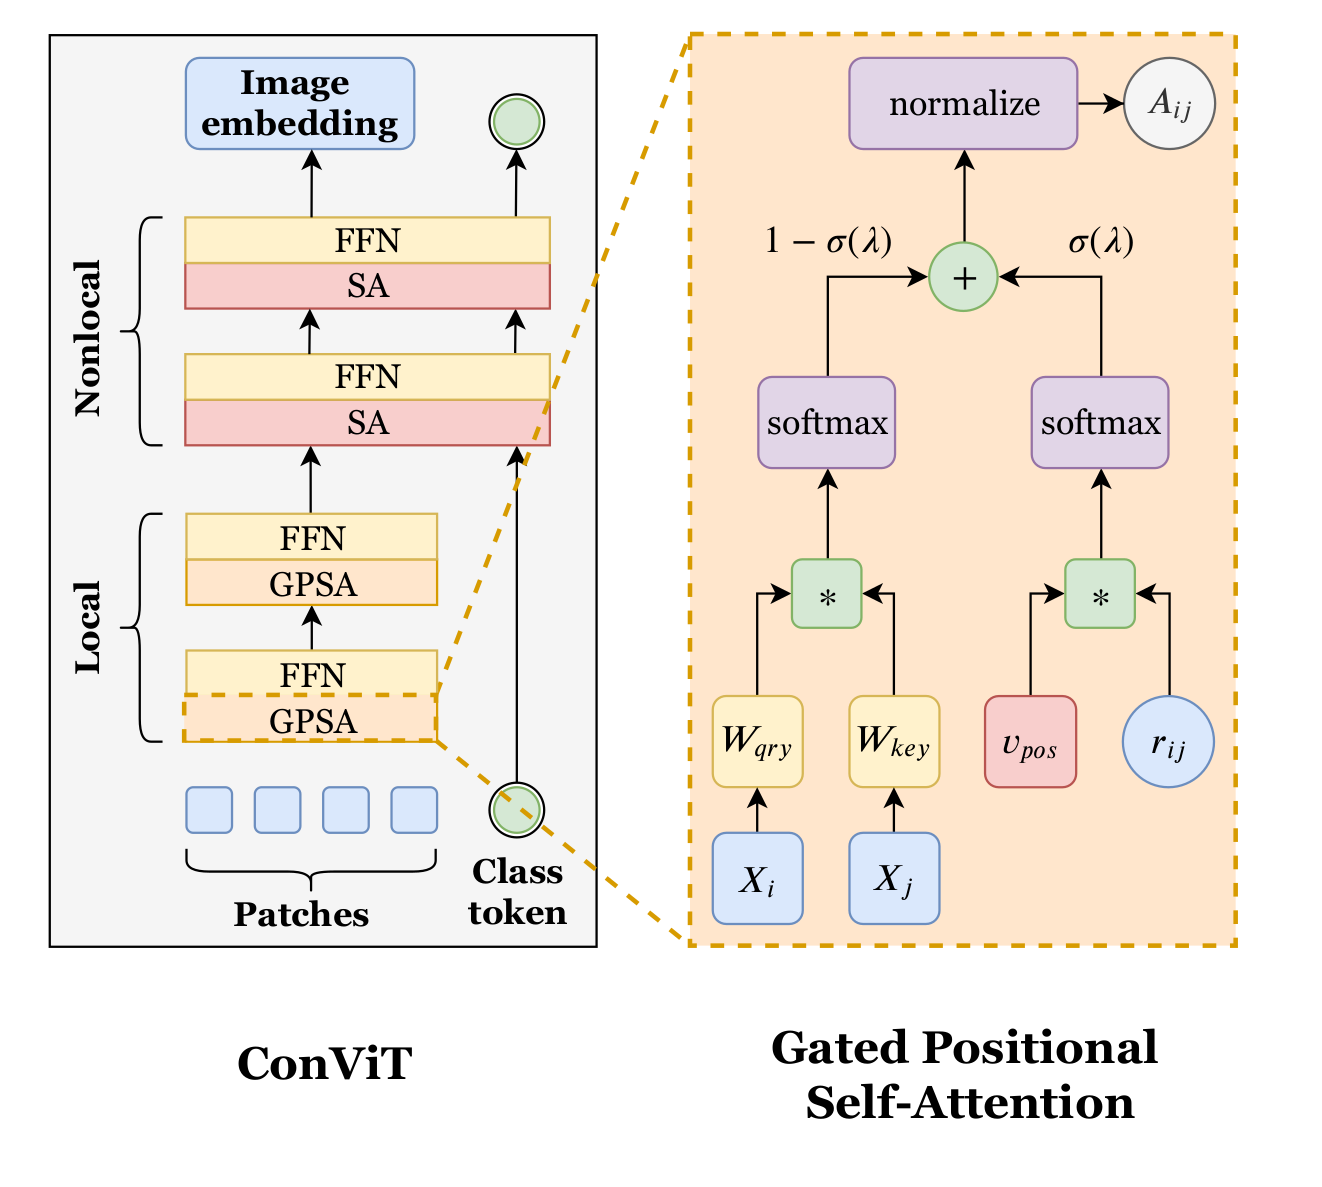
\includegraphics[width=0.3\textwidth]{figures/research_methadology/ConViT_model.png}
    \caption{ConViT GPSA Diagram \cite{DAscoli2021}}
    \label{fig:ConViT model}
\end{figure}

We train a true hybrid model CvT which maps convolutional layers onto attention patches, which does not have pre-trained weights available. The model architecture can be seen in figure \ref{fig:CvT}: 

\begin{figure}[ht!]
    \centering
    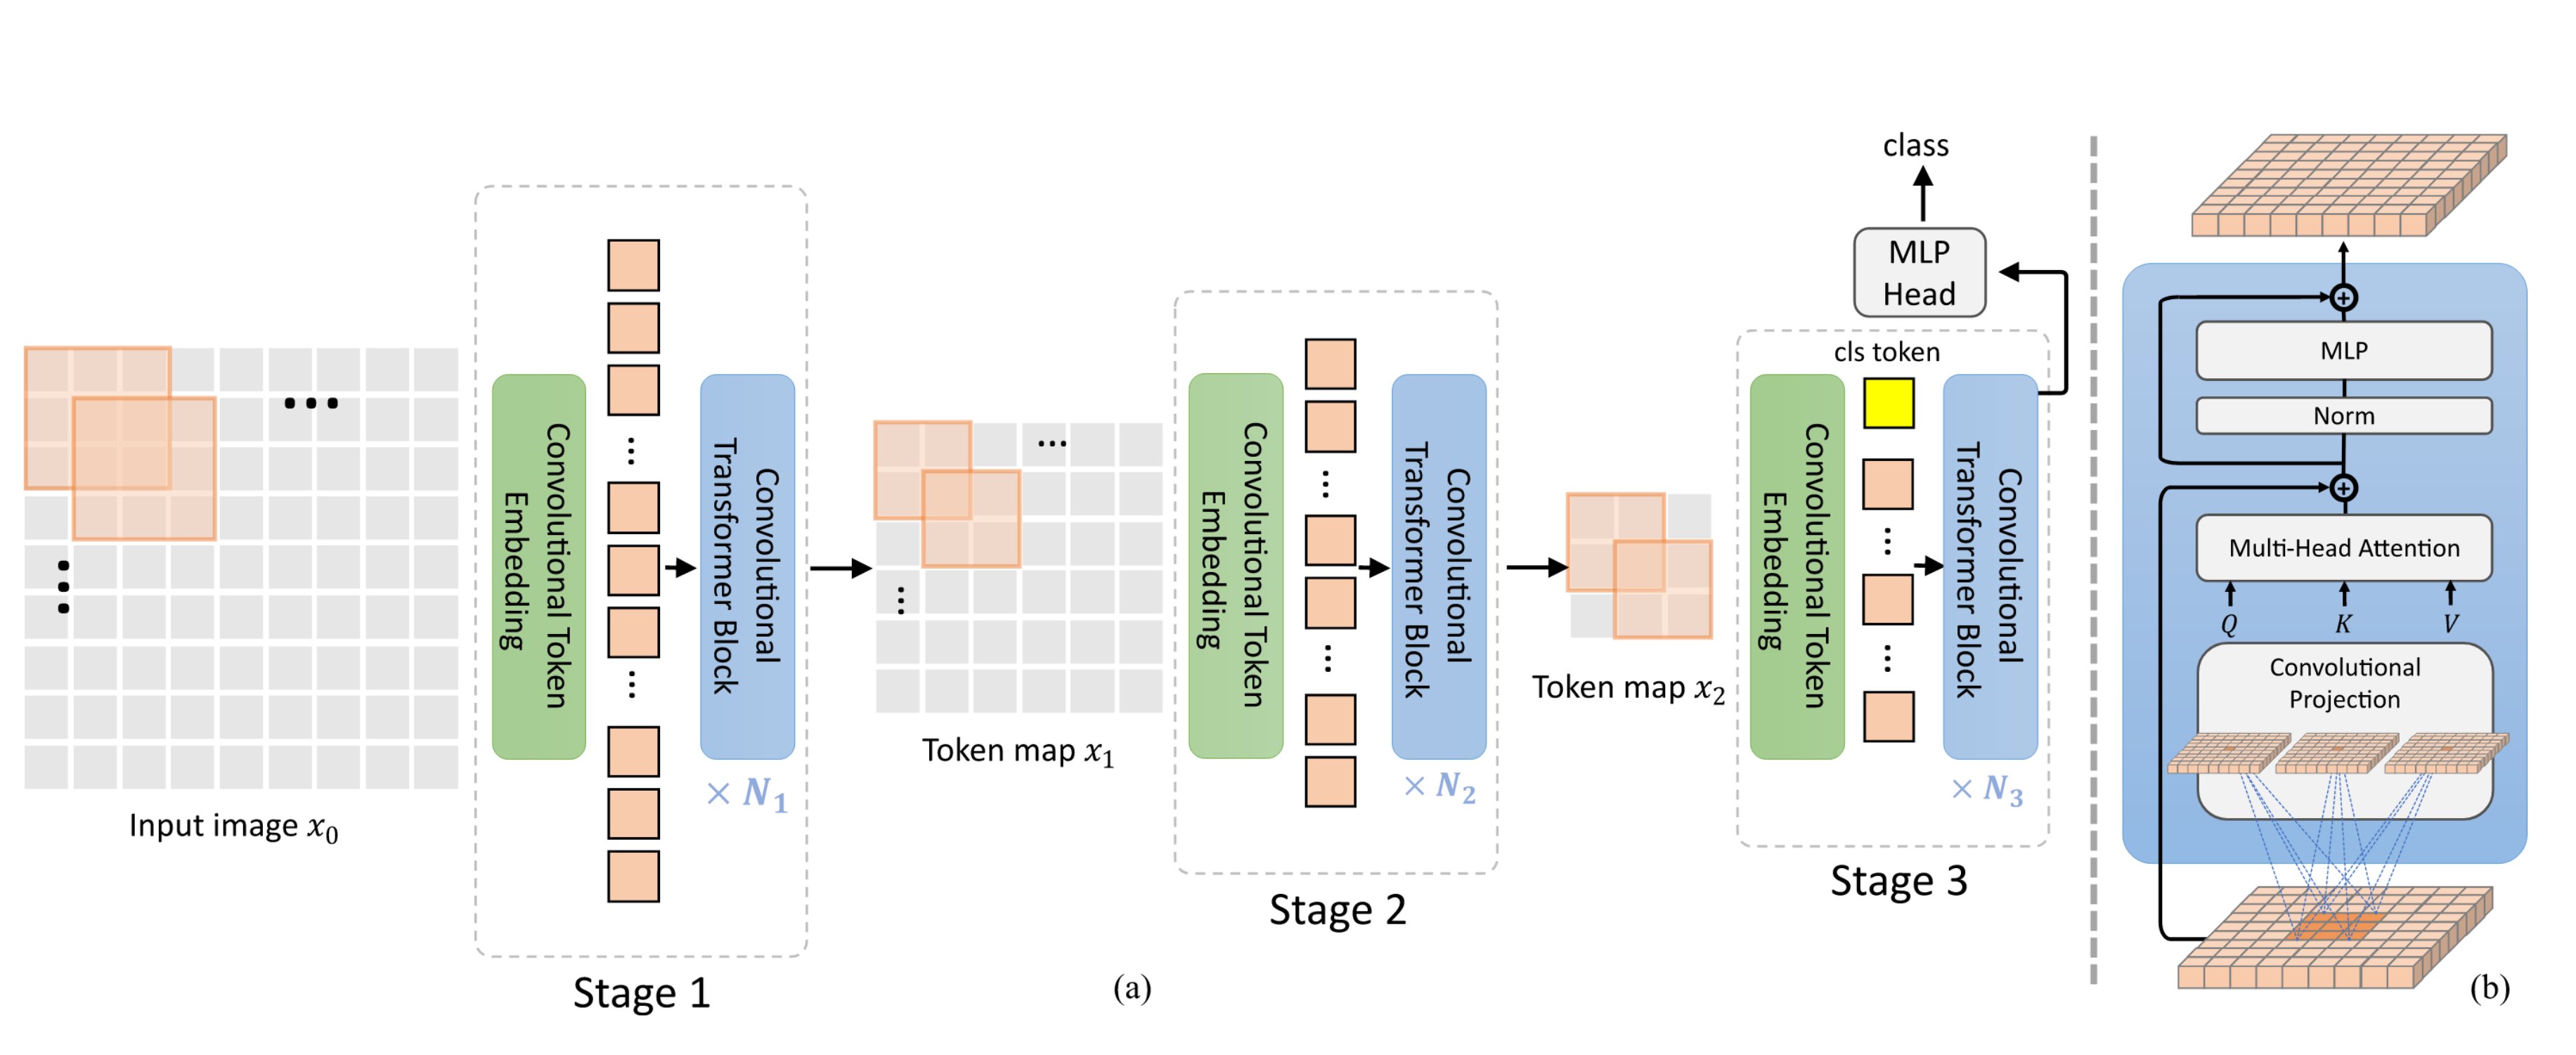
\includegraphics[width=0.6\textwidth]{figures/research_methadology/CViT.png}
    \caption{CvT Architecture and Pipeline \cite{Wu2021} }
    \label{fig:CvT}
\end{figure}

This provides metrics on a model that does not have a mechanism for switching between convolution and self attention, but incorporates \textit{as is}.

We train ConViT as an architecture that introduces convolutions as softer biases, where architecture is a positional layer that can be initialised to allow convolution initialisation of attention heads, with a one-to-one mapping. 



\subsection{Addressing Class Imbalance}

%n_samples / (n_classes * np.bincount(y))%
When thresholded into positive and negative image classes, the AVA dataset is heavily imbalanced towards the positive class with ration of (0.43:1). 

There are approaches to addressing class imbalance that involve defining a loss function and using balanced accuracy during training. However, we found that this was overly complex for a binary classification problem. Therefore, to address class imbalance during the training of ResNet $\in \{18,50,152\}$, we employed a data sampler to over sample the minority class during training. This further enabled repeated augmentation of the minority class which would not be possible if using a loss function. Class weights for the data-sampler are given by \ref{eq:class weights}.

\begin{figure}[ht]
    \centering
    \begin{subfigure}[b]{0.25\textwidth}
    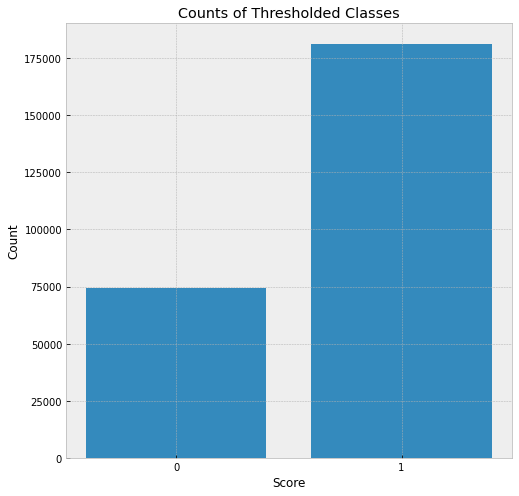
\includegraphics[height=\textwidth]{figures/research_methadology/imballance.png}
    \caption{Binary Class (Thresholded)}
    \label{fig:imbalance}
    \end{subfigure}
    \hspace{5mm}
    \begin{subfigure}[b]{0.25\textwidth}
    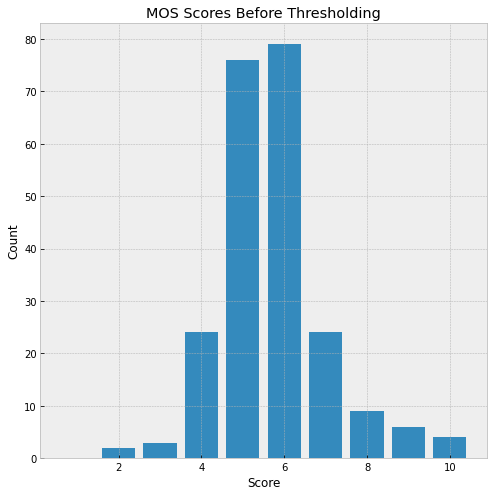
\includegraphics[height=\textwidth]{figures/research_methadology/mos counts.png}
    \caption{MOS Scores}
    \end{subfigure}
    \hspace{5mm}
    \begin{subfigure}[b]{0.25\textwidth}
    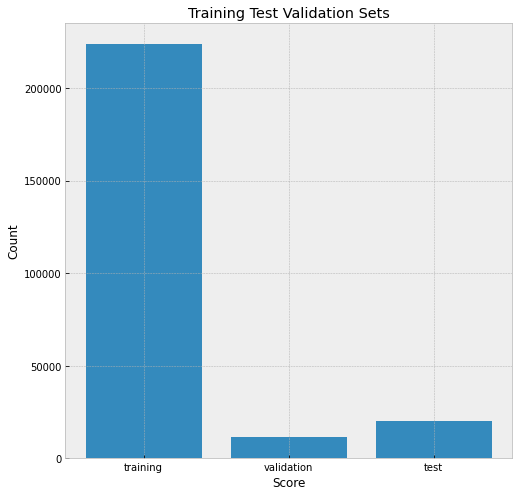
\includegraphics[height=\textwidth]{figures/research_methadology/test trian validation.png}
    \caption{Training, Validation, Test}
    \label{fig:test train}
    \end{subfigure}
    \caption{Class Imbalance and Test Training Validation Splits}
    \label{fig:class imballance}
    \end{figure}

\subsection{Research Methodology Summary}


We apply domain adaptation transfer learning, and train both baseline models (ResNets) to enable side-by-side comparison of ViTs, CvT's and CNNs, adding a fully connected \textit{linear} layer which outputs a 2D vector of $n \times c$ elements, for each class corresponds to a number of classes $y = xA^T +b $ where $A^T$ is the transposed input of the preceding layer; $b$ is some learnable bias. 

For training (batch-wise), validation (set-wise), and test (set-wise) inference, we apply a softmax function to produce class probables of the linear layer. We threshold data into binary classes from a continuous probability distribution that is calculated for each image based on a total number of votes, where each image receives an average of 210 votes. 

Thresholding given by eq. \ref{eq:threshold} is standard across IAQA literature on the AVA bench marking dataset. We also perform a grid search to establish a new hyper parameter, introduced by \cite{DAscoli2021} \textit{locality strength}. All models are pre-trained on ImageNet1k, and we train all models for 10 epochs with all layers unfrozen (trainable).

We try to apply a range of data augmentation techniques as part of training, which is doubly important as we have employed a data sampler that oversimplifies the minority class. We also outline a case for implementing convolution to introduce a soft inductive bias to the CvT's training to see if this makes the best of both transformers and CNNs, and also show how two very different models (CNNs) and ViTs learn.